\apendice{Documentación de usuario}\label{anex:D}

\section{Introducción}
Este documento detalla cómo un usuario puede utilizar la aplicación.
\section{Requisitos de usuarios}
Los requisitos para poder utilizar la aplicación son:
\begin{itemize}
	\tightlist
	\item Que la aplicación esté desplegada en algún servidor. En este caso se encuentra desplegada en \url{https://evolution-metrics-v2.herokuapp.com/}.
	\item Disponer de conexión a internet (o al servidor donde esté alojada la aplicación) y tener instalado un navegador web con el que poder acceder a la aplicación. Se recomienda en sus versiones lo más actualizadas posible los siguientes navegadores:
	\begin{itemize}
		\tightlist
		\item \textit{Google Chrome}
		\item \textit{Mozilla Firefox}
		\item \textit{Microsoft Edge}
		\item \textit{Opera}
		\item \textit{Safari}
	\end{itemize}
\end{itemize}

\section{Instalación}
Al tratarse de una aplicación web, esta no requiere instalación, basta con que el usuario acceda a la url de la aplicación desplegada. Además, si 

\section{Manual del usuario}
Para la utilización de la aplicación es necesario conectarse a las forjas disponibles (\textit{GitHub} y \textit{GitLab}), tras esto la aplicación recibe como entrada los datos de diferentes repositorios, calcula las métricas para los mismos y permite comparar los repositorios utilizando el cálculo estadístico de cuartiles.

\subsection{Conceptos}
Se deben conocer los siguientes conceptos:

\textbf{\textit{Medición}}

La medición es un proceso en el que se asignan números o símbolos a atributos de entidades del mundo real, de tal forma que los caracteriza a través de reglas. En nuestro caso realizamos mediciones de diferentes aspectos de los repositorios de software.

\textbf{\textit{Métrica}}

Medida cuantitativa del grado en que un sistema, componente o proceso posee un atributo dado (\textit{IEEE, 1993}).

\textbf{\textit{Indicador}}

Métrica o combinación de métricas que proporcionan una visión profunda del proceso, del proyecto o del producto.

\textbf{\textit{Métrica de evolución}}

Es una métrica que mide un atributo del proceso de desarrollo de un producto software.

\textbf{\textit{Evaluación}}

Consiste en determinar el estado de un proyecto en relación con otros proyectos de la misma naturaleza es uno de los objetivos clave del proceso de medición.

\textbf{\textit{Proyecto (software)}}

Proyecto en el cual se desarrolla un producto software.

\textbf{\textit{Repositorio de código}}

Lugar dónde se almacena el código de un proyecto software. A menudo cuentan con un sistema de control de versiones.

\textbf{\textit{Forja de repositorios}}

Lugar dónde se almacenan múltiples repositorios de código tanto públicos como privados de gran cantidad de usuarios o grupos. Cuentan con múltiples sistemas que facilitan la comunicación entre los desarrolladores y mejoran el soporte al usuario. Este proyecto se encuentra alojado en la forja \textit{GitHub}.

\textbf{\textit{Sistema de control de versiones (\textit{VCS - Version Control System})}}

Sistema que registra los cambios que se producen sobre los ficheros de un proyecto software almacenados en un repositorio de código.

\textbf{\textit{Sistema de seguimiento de incidencias (\textit{Issue tracking system})}}

Sistema que gestiona las diferentes tareas o incidentes que se definen en un proyecto software y que pueden ser asignadas a colaboradores del proyecto. En este proyecto se ha empleado el sistema \textit{GitHub Issues}.

\subsubsection{Las métricas que se gestionan en la aplicación}

Además de los conceptos anteriores, para comprender la aplicación y poder sacarle partidos, se tienen que conocer las métricas que ésta calcula y saber interpretarlas. La métricas proceden de la Master Tesis titulada \textit{sPACE: Software Project Assessment in the Course of Evolution} \cite{ratzinger_space:_2007} a las que se han añadido nuevas métricas relacionas con la Integración y Despliegue continuos:


Las métricas con las que se trabaja en la aplicación son las siguientes:

\textbf{\underline{I1 - Número total de \textit{issues} (incidencias)}}

\begin{itemize}
	\item \textbf{Categoría}: Proceso de Orientación
	\item \textbf{Descripción}: Número total de \textit{issues} creadas en el repositorio
	\item \textbf{Propósito}: ¿Cuántas \textit{issues} se han definido en el repositorio?
	\item \textbf{Fórmula}: $NTI$. \textit{NTI = número total de \textit{issues}}
	\item \textbf{Fuente de medición}: Proyecto en una plataforma de desarrollo colaborativo.
	\item \textbf{Interpretación}: $NTI \geq 0$. Valores bajos indican que no se utiliza un sistema de seguimiento de incidencias, podría ser porque el proyecto acaba de comenzar
	\item \textbf{Tipo de escala}: Absoluta
	\item \textbf{Tipo de medida}: \textit{NTI = Contador}
\end{itemize}

\textbf{\underline{I2 - \textit{Commits} (cambios) por \textit{issue}}}

\begin{itemize}
	\item \textbf{Categoría}: Proceso de Orientación
	\item \textbf{Descripción}: Número de \textit{commits} por \textit{issue}
	\item \textbf{Propósito}: ¿Cuál es el volumen medio de trabajo de las \textit{issues}?
	\item \textbf{Fórmula}: $CI = \frac{NTC}{NTI}$. \textit{CI = Cambios por \textit{issue}, NTC = Número total de \textit{commits}, NTI = Número total de \textit{issues}}
	\item \textbf{Fuente de medición}: Proyecto en una plataforma de desarrollo colaborativo.
	\item \textbf{Interpretación}: $CI \geq 1$, Lo normal son valores altos. Si el valor es menor que uno significa que hay desarrollo sin documentar.
	\item \textbf{Tipo de escala}: Ratio 
	\item \textbf{Tipo de medida}: \textit{NTC, NTI = Contador}
\end{itemize}

\textbf{\underline{I3 - Porcentaje de \textit{issues} cerradas}}

\begin{itemize}
	\item \textbf{Categoría}: Proceso de Orientación
	\item \textbf{Descripción}: Porcentaje de \textit{issues} cerradas
	\item \textbf{Propósito}: ¿Qué porcentaje de \textit{issues} definidas en el repositorio se han cerrado?
	\item \textbf{Fórmula}: $PIC = \frac{NTIC}{NTI}*100$. \textit{PIC = Porcentaje de \textit{issues} cerradas, NTIC = Número total de \textit{issues} cerradas, NTI = Número total de \textit{issues}}
	\item \textbf{Fuente de medición}: Proyecto en una plataforma de desarrollo colaborativo.
	\item \textbf{Interpretación}: $0 \leq PIC \leq 100$. Cuanto más alto mejor
	\item \textbf{Tipo de escala}: Ratio
	\item \textbf{Tipo de medida}: \textit{NTI, NTIC = Contador}
\end{itemize}

\textbf{\underline{TI1 - Media de días en cerrar una \textit{issue}}}

\begin{itemize}
	\item \textbf{Categoría}: Constantes de tiempo
	\item \textbf{Descripción}:  Media de días en cerrar una \textit{issue}
	\item \textbf{Propósito}: ¿Cuánto se suele tardar en cerrar una \textit{issue}? 
	\item \textbf{Fórmula}: $MDCI = \frac{\sum_{i=0}^{NTIC}DCI_i}{NTIC}$. \textit{MDCI = Media de días en cerrar una \textit{issue}, NTIC = Número total de \textit{issues} cerradas, DCI = Días en cerrar la \textit{issue}}
	\item \textbf{Fuente de medición}: Proyecto en una plataforma de desarrollo colaborativo.
	\item \textbf{Interpretación}: $MDCI \geq 0$. Cuanto más pequeño mejor. Si se siguen metodologías ágiles de desarrollo iterativo e incremental como \textit{SCRUM}, la métrica debería indicar la duración del \textit{sprint} definido en la fase de planificación del proyecto. En \textit{SCRUM} se recomiendan duraciones del \textit{sprint} de entre una y seis semanas, siendo recomendable que no exceda de un mes \cite{scrum_master_scrum_2019}.
	\item \textbf{Tipo de escala}: Ratio
	\item \textbf{Tipo de medida}: \textit{NTI, NTIC = Contador}
\end{itemize}

\textbf{\underline{TC1 - Media de días entre \textit{commits}}}

\begin{itemize}
	\item \textbf{Categoría}: Constantes de tiempo
	\item \textbf{Descripción}: Media de días que pasan entre dos \textit{commits} consecutivos
	\item \textbf{Propósito}: ¿Cuántos días suelen pasar desde un \textit{commit} hasta el siguiente?
	\item \textbf{Fórmula}: $MDC = \frac{\sum_{i=1}^{NTC} TC_i - TC_{i-1}}{NTC}$. $TC_i - TC_{i-1}$ en días; \textit{MDC = Media de días entre cambios, NTC = Número total de \textit{commits}, TC = Tiempo de \textit{commit}}
	%$MDEC = [Sumatorio de (TCi-TCj) desde i=1, j=0 hasta i=NTC] / NTC. NTC = Número total de commits, TC = Tiempo de Commit$ 
	\item \textbf{Fuente de medición}: Proyecto en una plataforma de desarrollo colaborativo.
	\item \textbf{Interpretación}: $MDEC \geq 0$. Cuanto más pequeño mejor. Se recomienda no superar los 5 días.
	\item \textbf{Tipo de escala}: Ratio
	\item \textbf{Tipo de medida}: \textit{NTC = Contador; TC = Tiempo}
\end{itemize}

\textbf{\underline{TC2 - Días entre primer y último \textit{commit}}}

\begin{itemize}
	\item \textbf{Categoría}: Constantes de tiempo
	\item \textbf{Descripción}: Días transcurridos entre el primer y el último \textit{commit} 
	\item \textbf{Propósito}: ¿Cuantos días han pasado entre el primer y el último \textit{commit}?
	\item \textbf{Fórmula}: $DEPUC = TC2- TC1$. $TC2- TC1$ en días;  \textit{DEPUC = Días entre primer y último \textit{commit}, TC2 = Tiempo de último \textit{commit}, TC1 = Tiempo de primer \textit{commit}}
	\item \textbf{Fuente de medición}: Proyecto en una plataforma de desarrollo colaborativo.
	\item \textbf{Interpretación}: $DEPUC \geq 0$. Cuanto más alto, más tiempo lleva en desarrollo el proyecto. En procesos software empresariales se debería comparar con la estimación temporal de la fase de planificación. 
	\item \textbf{Tipo de escala}: Absoluta
	\item \textbf{Tipo de medida}: \textit{TC = Tiempo}
\end{itemize}

\textbf{\underline{TC3 - Ratio de actividad de \textit{commits} por mes}}

\begin{itemize}
	\item \textbf{Categoría}: Constantes de tiempo
	\item \textbf{Descripción}: Muestra el número de \textit{commits} relativos al número de meses
	\item \textbf{Propósito}:¿Cuál es el número medio de cambios por mes?
	\item \textbf{Fórmula}: $RCM = \frac{NTC}{NM}$. \textit{RCM = Ratio de cambios por mes, NTC = Número total de \textit{commits}, NM = Número de meses que han pasado durante el desarrollo de la aplicación}
	\item \textbf{Fuente de medición}: Proyecto en una plataforma de desarrollo colaborativo.
	\item \textbf{Interpretación}: $RCM > 0$. Cuanto más alto mejor
	\item \textbf{Tipo de escala}: Ratio
	\item \textbf{Tipo de medida}: \textit{NTC = Contador}
\end{itemize}

\textbf{\underline{C1 - Cambios pico}}

\begin{itemize}
	\item \textbf{Categoría}: Constantes de tiempo
	\item \textbf{Descripción}: Número de \textit{commits} en el mes que más \textit{commits} se han realizado en relación con el número total de \textit{commits}
	\item \textbf{Propósito}: ¿Cuál es la proporción de trabajo realizado en el mes con mayor número de cambios?
	\item \textbf{Fórmula}: $CP = \frac{NCMP}{NTC}$. \textit{CP = Cambios pico, NCMP = Número de \textit{commits} en el mes pico, NTC = Número total de \textit{commits}}
	\item \textbf{Fuente de medición}: Proyecto en una plataforma de desarrollo colaborativo.
	\item \textbf{Interpretación}: $0 \leq CCP \leq 1$. Mejor valores intermedios. Se recomienda no superar el 40\% del trabajo en un mes.
	\item \textbf{Tipo de escala}: Ratio
	\item \textbf{Tipo de medida}: \textit{NCMP, NTC = Contador}
\end{itemize}

\textbf{\underline{IC1 - Número total de \textit{jobs} ejecutados}}
\begin{itemize}
	\item \textbf{Categoría}: \textit{CICD}
	\item \textbf{Descripción}: Número de \textit{jobs} ejecutados en el proyecto.
	\item \textbf{Propósito}: ¿Cuál es el número total de de \textit{jobs} ejecutados con éxito en el proyecto?
	\item \textbf{Fórmula}: $NJE =$ \textit{número total de jobs}.
	\item \textbf{Fuente de medición}: Proyecto en una plataforma de desarrollo colaborativo.
	\item \textbf{Interpretación}: $NJE \geq 0$. Un valor de cero indica que el proyecto no tiene integración y despliegues continuos y no se ha realizado ningún trabajo automatizado de despliegue.
	\item \textbf{Tipo de escala}: Absoluta
	\item \textbf{Tipo de medida}: \textit{NJE = Contador}
\end{itemize}

\textbf{\underline{IC2 - Número de \textit{Jobs} ejecutados el último año}}
\begin{itemize}
	\item \textbf{Categoría}: \textit{CICD}
	\item \textbf{Descripción}: Número de \textit{jobs} ejecutados en el último año (últimos 365 días).
	\item \textbf{Propósito}: ¿Cuál es el número total de \textit{jobs} ejecutados con éxito en el proyecto durante el año previo?
	\item \textbf{Fórmula}: $NJELY =$ \textit{número total de jobs ejecutados el útimo año}.
	\item \textbf{Fuente de medición}: Proyecto en una plataforma de desarrollo colaborativo.
	\item \textbf{Interpretación}: $NJELY \geq 0$. Un valor de cero indica que en el proyecto no se ha realizado ningún trabajo automatizado de despliegue durante el último año.
	\item \textbf{Tipo de escala}: Absoluta
	\item \textbf{Tipo de medida}: \textit{NJELY = Contador}
\end{itemize}

\textbf{\underline{IC3 - \textit Número de tipos diferentes de{jobs} ejecutados}}
\begin{itemize}
	\item \textbf{Categoría}: \textit{CICD}
	\item \textbf{Descripción}: Número de tipos diferentes de \textit{jobs} ejecutados en el proyecto.
	\item \textbf{Propósito}: ¿Cuál es el número total de tipos de \textit{jobs} ejecutados con éxito en el proyecto?
	\item \textbf{Fórmula}: $NTJE =$ \textit{número total de tipos diferentes de jobs ejecutados en el proyecto}.
	\item \textbf{Fuente de medición}: Proyecto en una plataforma de desarrollo colaborativo.
	\item \textbf{Interpretación}: $NTJE \geq 0$. Un valor de cero indica que el proyecto no tiene integración y despliegues continuos y no se ha realizado ningún trabajo automatizado de despliegue.
	\item \textbf{Tipo de escala}: Absoluta
	\item \textbf{Tipo de medida}: \textit{NTJE = Contador}
\end{itemize}

\textbf{\underline{DC1 - \textit Número total de{releases}}}
\begin{itemize}
	\item \textbf{Categoría}: \textit{CICD}
	\item \textbf{Descripción}: Número de \textit{releases} lanzadas en el proyecto.
	\item \textbf{Propósito}: ¿Cuál es el número total de \textit{releases} del  proyecto?
	\item \textbf{Fórmula}: $NRR =$ \textit{número total de releases lanzadas en el proyecto}.
	\item \textbf{Fuente de medición}: Proyecto en una plataforma de desarrollo colaborativo.
	\item \textbf{Interpretación}: $NRR \geq 0$. Un valor de cero indica que aún no se ha lanzado ninguna \textit{release} del proyecto.
	\item \textbf{Tipo de escala}: Absoluta
	\item \textbf{Tipo de medida}: \textit{NRR = Contador}
\end{itemize}

\subsection{Arranque de la aplicación: Establecer una conexión a \textit{GitLab}}
Para poder añadir repositorios desde las forjas es necesario realizar una conexión a cada una de ellas a través de los botones que podemos encontrar en la parte superior derecha de la interfaz como se ve en la figura \ref{fig:AnexE-MN-Fig1}.

\begin{figure}[!h]
	\centering
	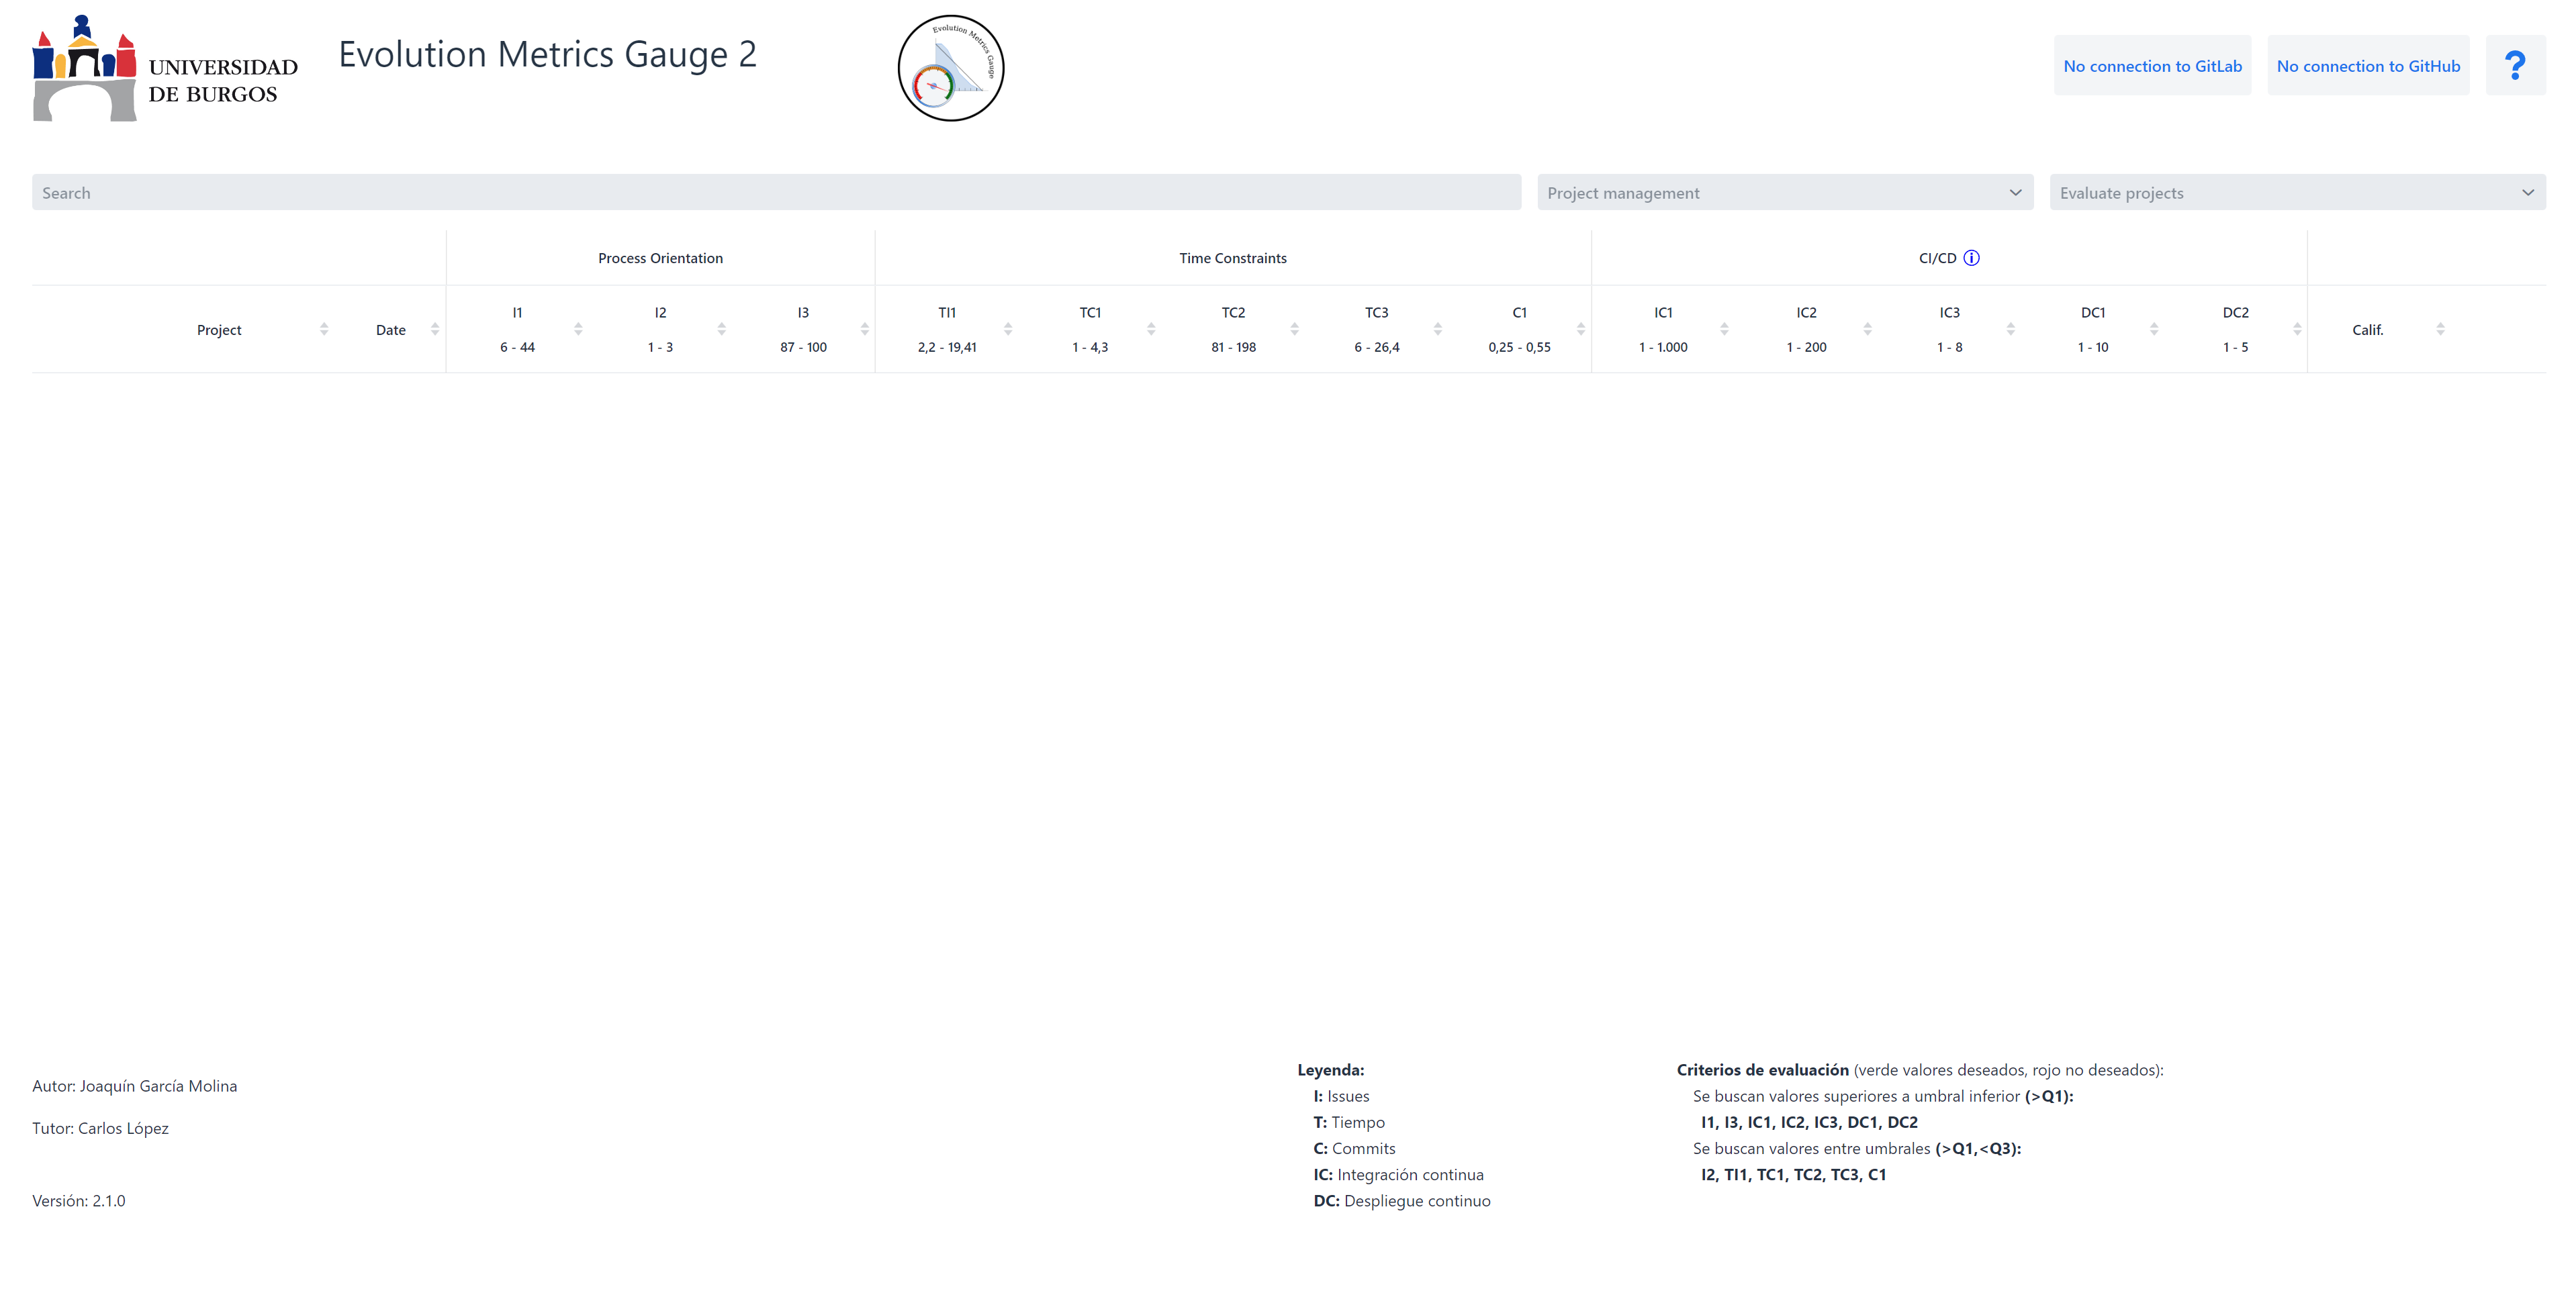
\includegraphics[width=1\textwidth]{AnexE-MN-Fig1}
	\caption{Botones de conexión}\label{fig:AnexE-MN-Fig1}
\end{figure}
\FloatBarrier

Para realizar la conexión con \textit{GitHub} debido a cómo trabaja su \textit{API} sólo podemos conectarnos utilizando un \textit{token} personal \footnote{Crear un \textit{token} de acceso personal para \textit{GitHub}: \url{https://docs.github.com/es/authentication/keeping-your-account-and-data-secure/creating-a-personal-access-token}}:
\begin{figure}[!h]
	\centering
	\begin{subfigure}{.45\textwidth}
		\centering
		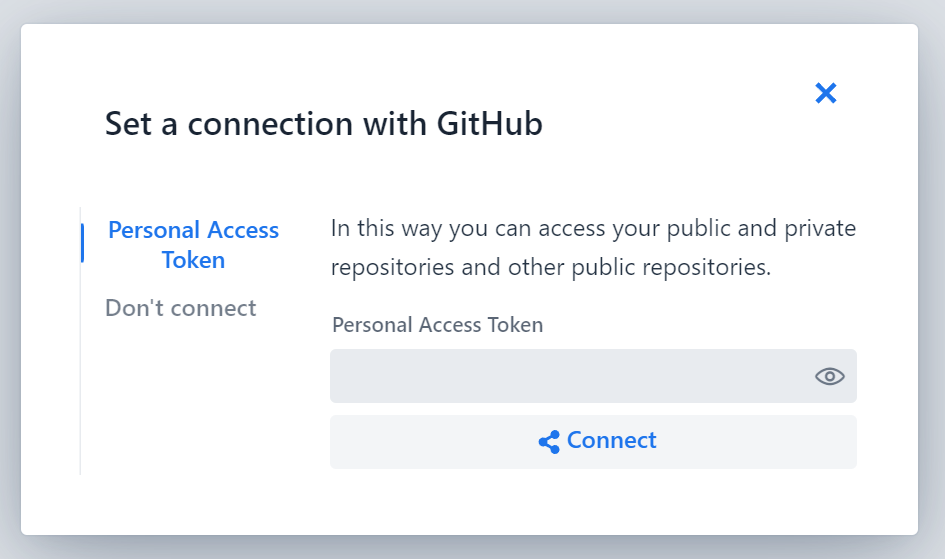
\includegraphics[width=\linewidth]{AnexE-MN-Fig1-5}
		\caption{Establecer conexión iniciando sesión mediante \textit{Personal Access Token}}
		\label{fig:dialogo-conexion_contraseña}
	\end{subfigure}\hfill
	\begin{subfigure}{.45\textwidth}
		\centering
		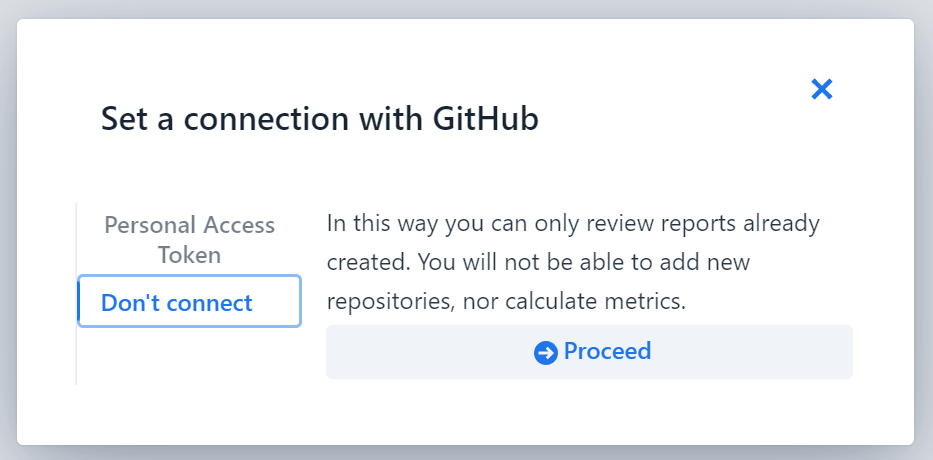
\includegraphics[width=\linewidth]{AnexE-MN-Fig1-6}
		\caption{No establecer conexión a \textit{GitHub}}
		\label{fig:dialogo-conexion_token}
	\end{subfigure}
	\caption{Conexión con \textit{GitHub}}
	\label{fig:AnexE-MN-Fig1}
\end{figure}


Para realizar la conexión con \textit{GitLab} tenemos cuatro opciones, mediante usuario y contraseña, mediante \textit{PA Token}  \footnote{Crear un \textit{token} de acceso personal para \textit{GitLab}: \url{https://docs.gitlab.com/ee/user/profile/personal_access_tokens.html}}, usar una conexión pública o utilizar la aplicación sin conexión:
		\label{fig:dialogo-conexion_token}:\\

\begin{figure}[!h]
	\centering
	\begin{subfigure}{.45\textwidth}
		\centering
		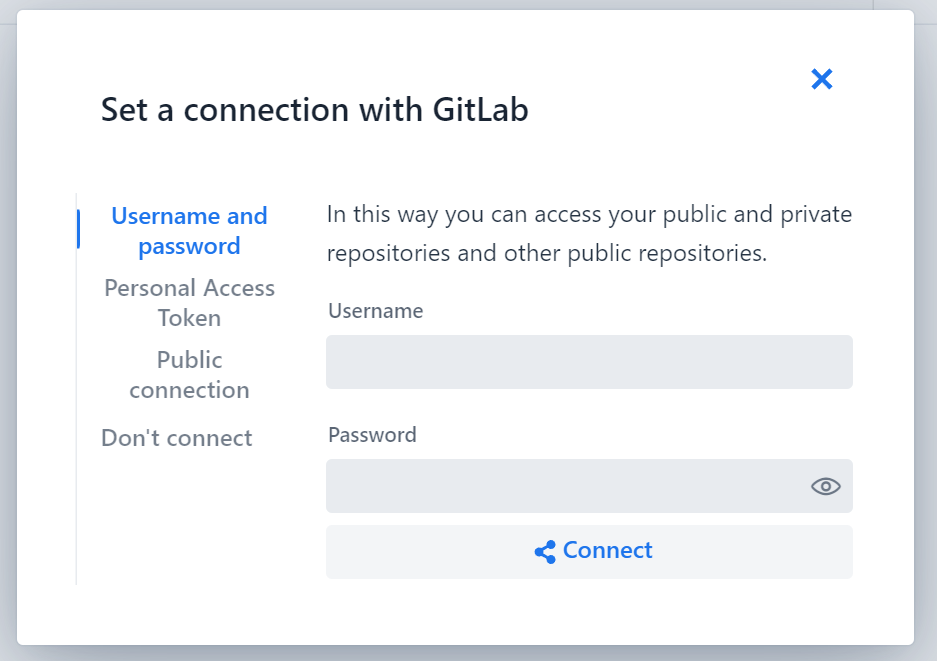
\includegraphics[width=\linewidth]{AnexE-MN-Fig1-1}
		\caption{Establecer conexión iniciando sesión mediante usuario y contraseña}
		\label{fig:dialogo-conexion_contraseña}
	\end{subfigure}\hfill
	\begin{subfigure}{.45\textwidth}
		\centering
		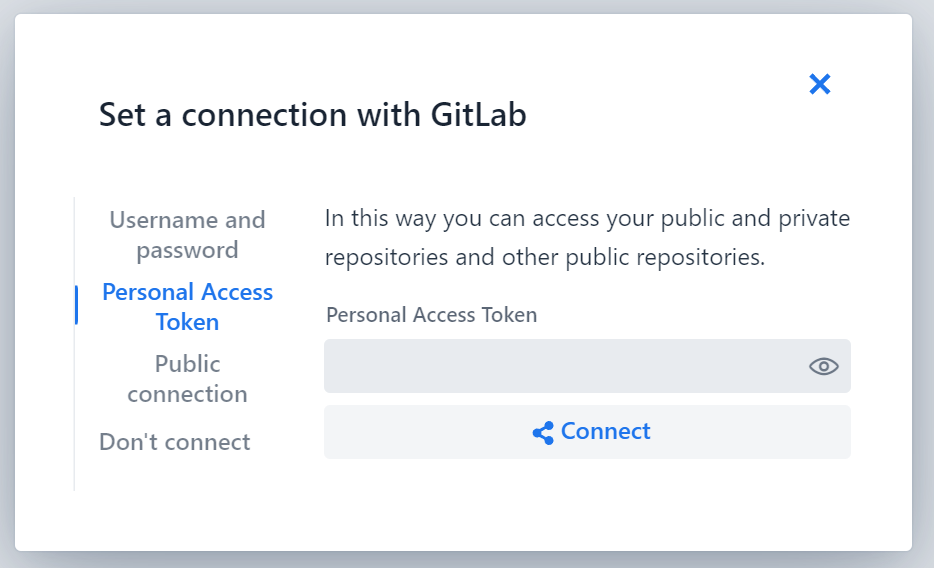
\includegraphics[width=\linewidth]{AnexE-MN-Fig1-2}
		\caption{Establecer conexión iniciando sesión mediante \textit{Personal Access Token}}
	\end{subfigure}
	\begin{subfigure}{.45\textwidth}
		\centering
		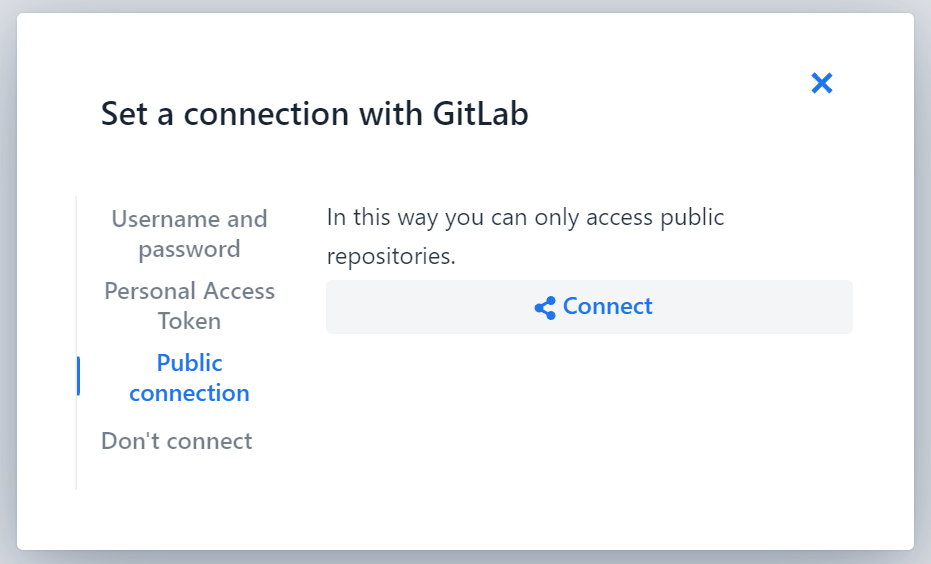
\includegraphics[width=\linewidth]{AnexE-MN-Fig1-3}
		\caption{Establecer una conexión publica}
		\label{fig:dialogo-conexion_publica}
	\end{subfigure}\hfill
	\begin{subfigure}{.45\textwidth}
		\centering
		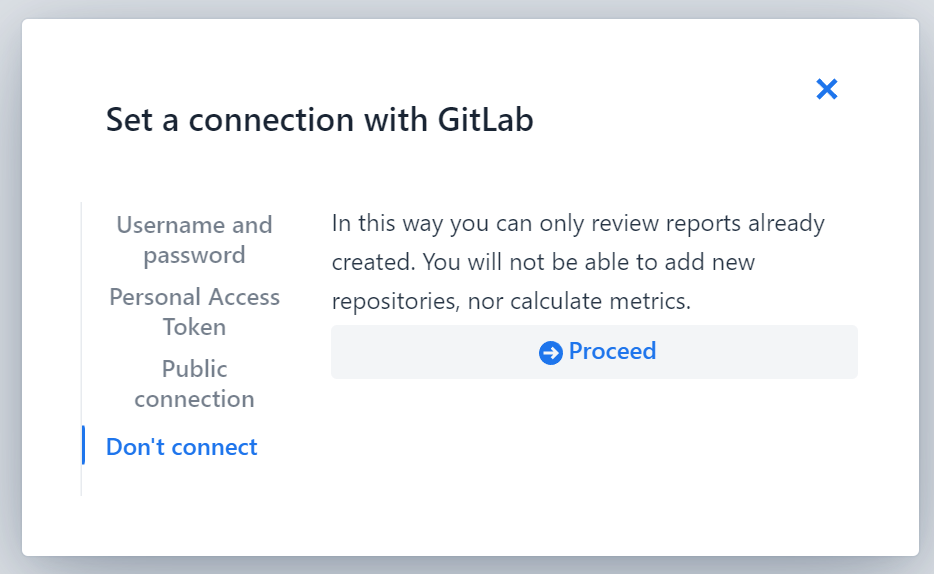
\includegraphics[width=\linewidth]{AnexE-MN-Fig1-4}
		\caption{No establecer conexión a \textit{GitLab}}
		\label{fig:dialogo-conexion_sin-conexion}
	\end{subfigure}
	\caption{Distintas formas de establecer una conexión con \textit{GitLab}}
	\label{fig:AnexE-MN-Fig1}
\end{figure}

\begin{description}
	\tightlist
	\item[Iniciar sesión en \textit{GitLab} mediante usuario y contraseña.] Se establece una conexión a \textit{GitLab} iniciando sesión mediante un nombre de usuario y una contraseña. De esta forma se puede acceder a todos los repositorios públicos y privados accesibles por el usuario. Ver figura \ref{fig:dialogo-conexion_contraseña}.
	\item[Iniciar sesión mediante \textit{Personal Access Token}.] Se establece una conexión iniciando sesión mediante un \textit{Personal Access Token}. De esta forma se puede acceder a todos los repositorios públicos y privados accesibles por usuario, como ocurría en el caso anterior. 
	Si se accede a \textit{GitLab} desde una \underline{cuenta externa} a \textit{GitLab} como \textit{Google} o \textit{GitHub}, esta opción es la única manera de iniciar sesión con su cuenta de \textit{GitLab}. Ver figura \ref{fig:dialogo-conexion_token}.\\
	\item[Usar una conexión pública hacia \textit{GitLab}.] Se establece una conexión pública a \textit{GitLab} sin iniciar sesión, por lo que solo se podrá acceder a repositorios públicos, no a los privados. Ver figura \ref{fig:dialogo-conexion_publica}.\\
	Además es importante indicar que no se calcularán las métricas relacionadas con \textit{CICD} ya que la \textit{API} de \textit{GitLab} no devuelve los valores necesarios para calcularlas con este tipo de conexión (se necesita alguna de las dos anteriores).
	\item[No utilizar ninguna conexión.] No se realizará ninguna conexión, de esta forma se impide al usuario añadir nuevos repositorios desde las dos forjas ni volver a calcular métricas de los proyectos existentes. Sin embargo, se permite gestionar los proyectos ya existentes, permitiendo su exportación e importación desde un fichero con extensión \ruta{.emr}. También se permite usar el sistema de perfil de métricas sin ninguna restricción: se puede crear un nuevo perfil, importar, exportar y utilizar el perfil por defecto de la aplicación. Ver figura \ref{fig:dialogo-conexion_sin-conexion}.
\end{description}

\newpage
\subsection{Página principal}

% \imagen{AnexE-MN-Fig1-bis}{Página principal}

Una vez establecidas las conexiones, se puede comenzar a trabajar con los repositorios como se observa en la figura \ref{fig:AnexE-MN-Fig1-bis}.

\begin{figure}[!h]
	\centering
	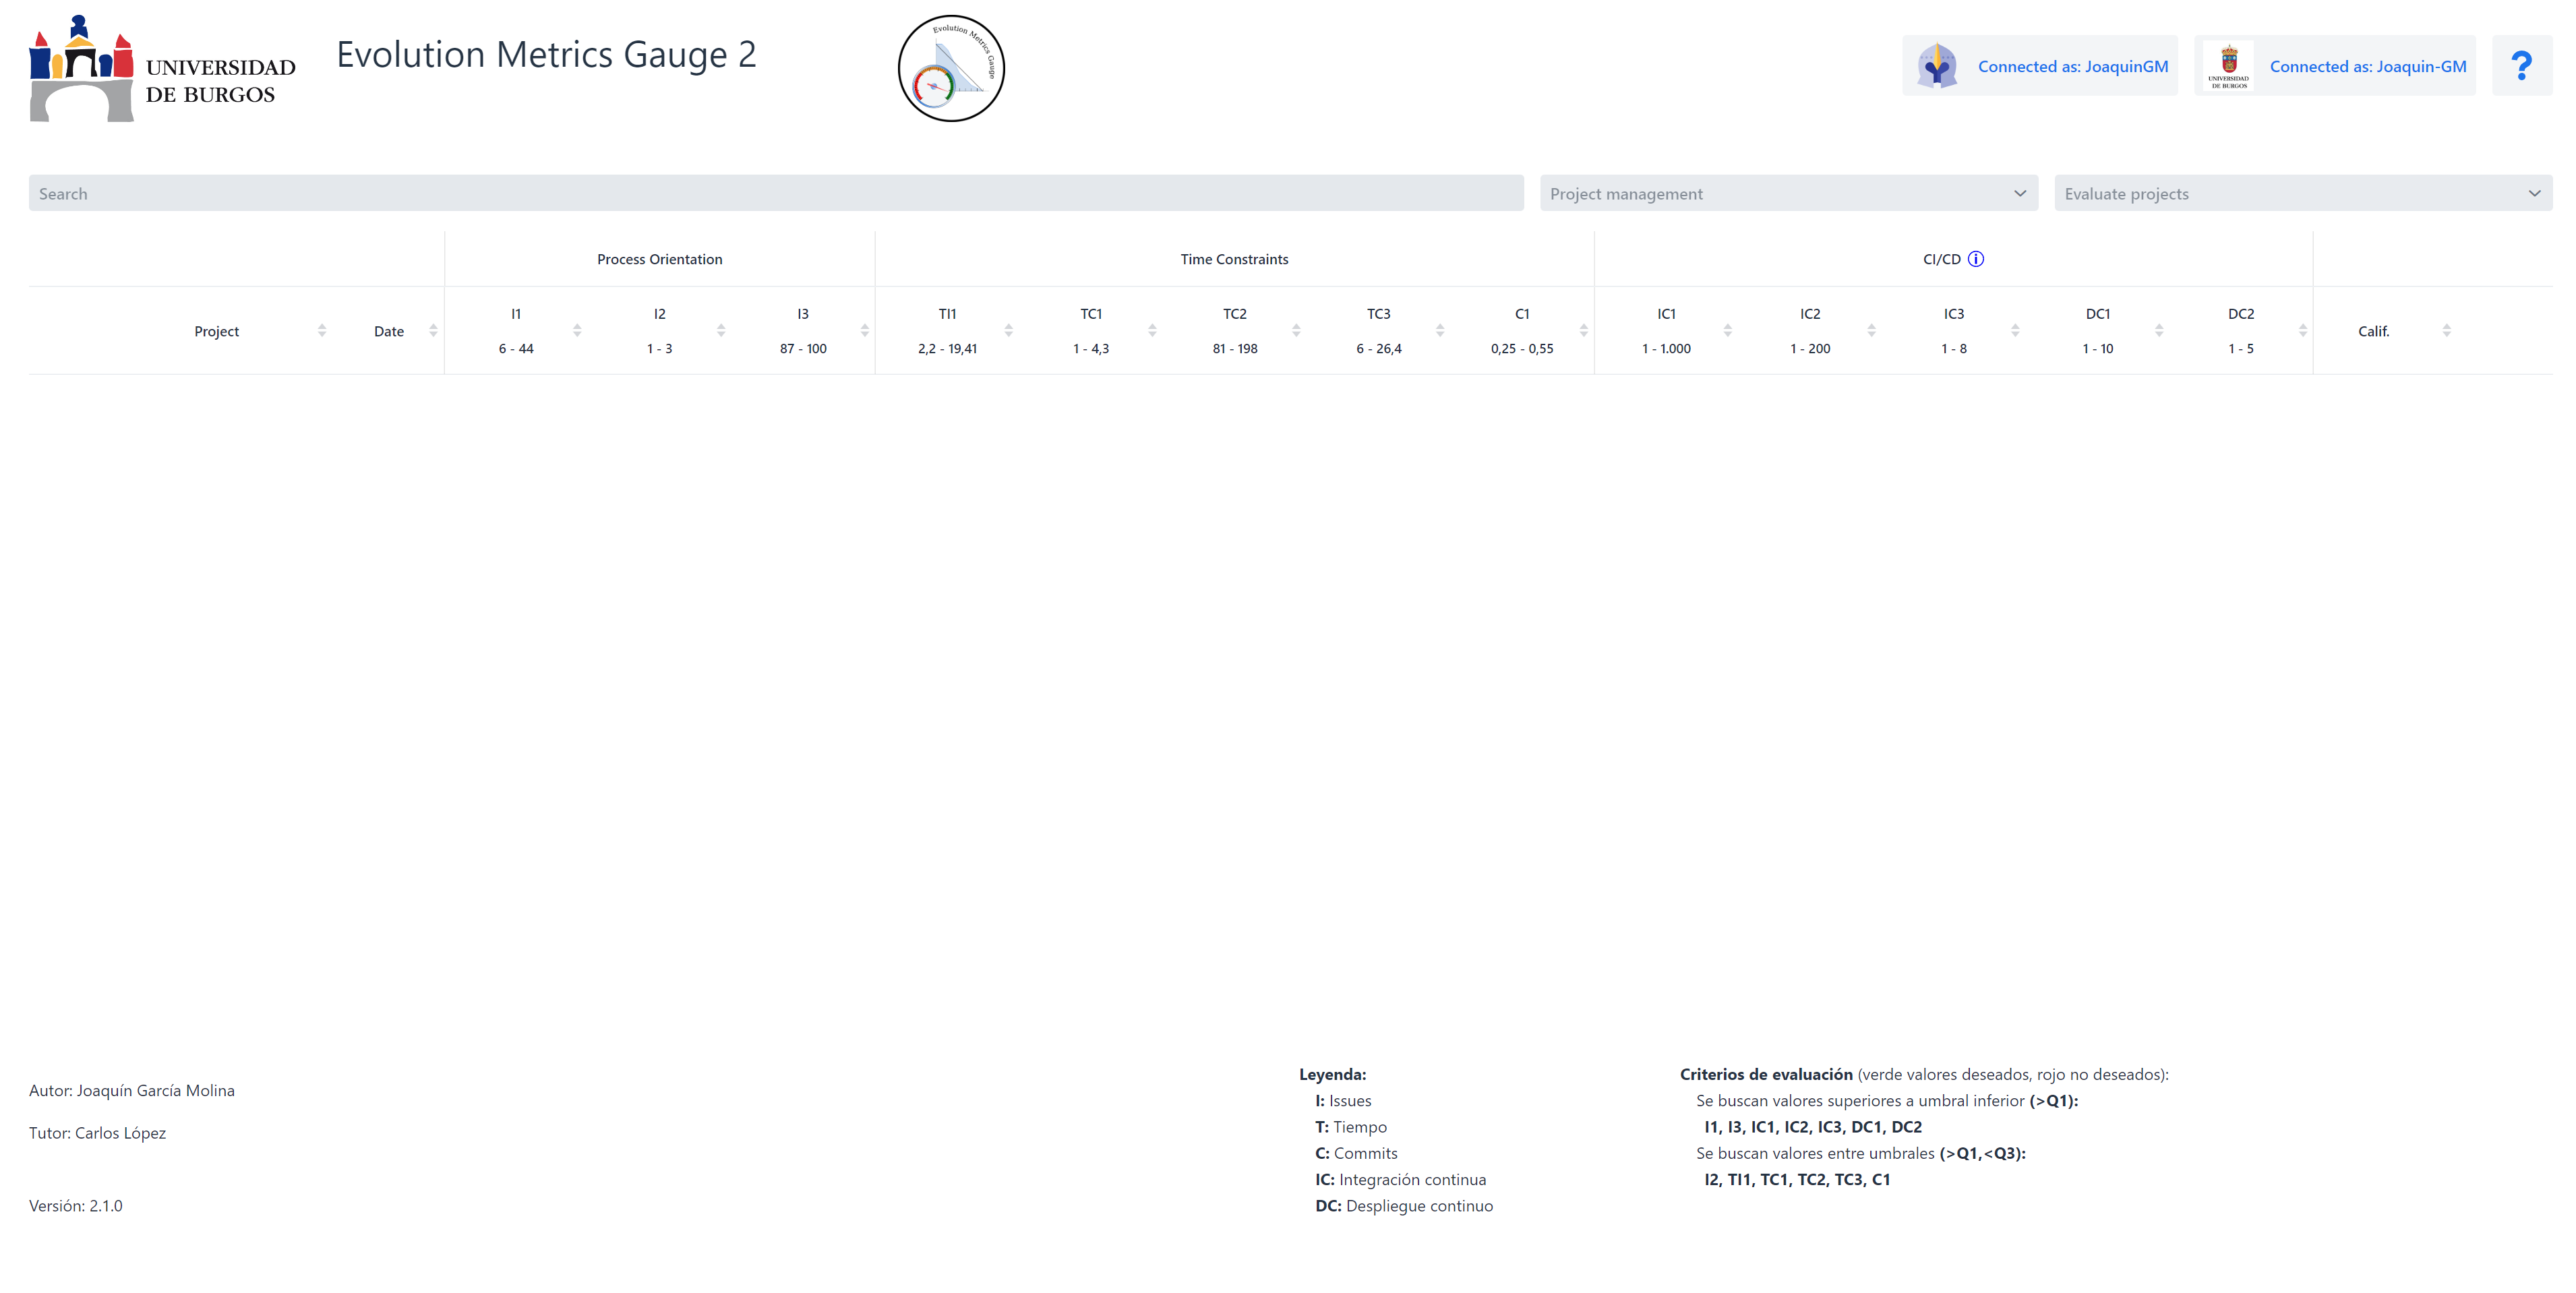
\includegraphics[width=1\textwidth]{AnexE-MN-Fig1-bis}
	\caption{Página principal}\label{fig:AnexE-MN-Fig1-bis}
\end{figure}
\FloatBarrier

\subsubsection{Cambiar el tipo de conexión}

En la parte superior se puede observar el botón de conexión, que indica el tipo de conexión actual.
\begin{itemize}
	\tightlist
	\item Si se ha iniciado sesión mediante usuario y contraseña o mediante un \textit{personal access token}, se mostrará la imágen del usuario y el texto: ``Connected as: <nombre de usuario>''
	\item Si se ha establecido una conexión pública, se mostrara el texto: ``Using a public connection''
	\item Y si no se ha establecido ninguna conexión, el texto mostrado será: ``No connection to GitHub/GitLab''.
\end{itemize}
Para cambiar el tipo de conexión es obligatorio cerrar (si existe), la conexión actual. Por ello, al pulsar sobre el botón de conexión, se muestra el diálogo de la figura \ref{fig:AnexE-MN-Fig4-1} si existe una conexión y el diálogo de la figura \ref{fig:AnexE-MN-Fig4-2} si no existe conexión. Al pulsar sobre ``\textit{Connect}'' o sobre ``\textit{Close connection}'', respectivamente, se abrirá alguno de los7 diálogos de conexión de la figura \ref{fig:AnexE-MN-Fig1}
\begin{figure}[!h]
	\centering
	\begin{subfigure}{.45\textwidth}
		\centering
		
\includegraphics[width=\linewidth]{AnexE-MN-Fig4-1}
		\caption{Cerrar conexión}
		\label{fig:AnexE-MN-Fig4-1}
	\end{subfigure}\hfill
	\begin{subfigure}{.45\textwidth}
		\centering
		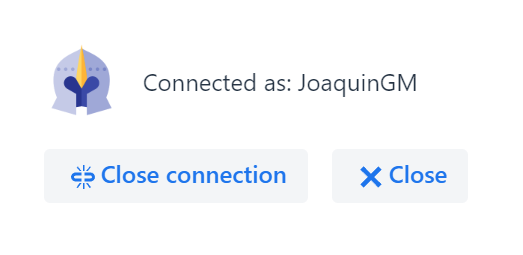
\includegraphics[width=\linewidth]{AnexE-MN-Fig4-3}
		\caption{Conectado como...}
		\label{fig:AnexE-MN-Fig4-1}
	\end{subfigure}\hfill
	\begin{subfigure}{.45\textwidth}
		\centering
		
\includegraphics[width=\linewidth]{AnexE-MN-Fig4-2}
		\caption{Sin conexión a \textit{GitLab}}
		\label{fig:AnexE-MN-Fig4-2}
	\end{subfigure}\hfill
	\begin{subfigure}{.45\textwidth}
		\centering
		
\includegraphics[width=\linewidth]{AnexE-MN-Fig4-4}
		\caption{Sin conexión a \textit{GitHub}}
		\label{fig:AnexE-MN-Fig4-2}
	\end{subfigure}\hfill
	\caption{Modificar tipo de conexión}
	\label{fig:AnexE-MN-Fig4}
\end{figure}

\newpage
\subsubsection{Botón de ayuda}
A la derecha del botón de conexión se encuentra un botón que da acceso a este manual en la Wiki del proyecto: \url{https://github.com/Joaquin-GM/GII_O_MA_19.07-Comparador-de-metricas-de-evolucion-en-repositorios-Software/wiki}.

\subsubsection{Listado de proyectos}
En la parte central de la interfaz principal se gestionan los proyectos. Consta de una barra de búsqueda, dos menús, y una tabla que visualiza las métricas de los proyectos que se añadan.

En el \textbf{cuadro de búsqueda} se filtrarán los repositorios por su nombre según se vaya escribiendo.

En el \textbf{menú de ``\textit{Project management}''} existen las siguientes opciones, como se muestra en la figura \ref{fig:AnexE-MN-Fig5-1}:
\begin{itemize}
	\item \textbf{\textit{Add new GitLab repository}.} Permite añadir un nuevo repositorio de \textit{GitLab} (disponible sólo con conexión). 
	
	\item \textbf{\textit{Add new GitHub repository}.} Permite añadir un nuevo repositorio de \textit{GitHub} (disponible sólo con conexión). 
	
	\item \textbf{\textit{Import}.} Permite importar proyectos a partir de un fichero previamente exportado.
	
	\item \textbf{\textit{Export}.} Permite exportar todos los proyectos existentes a un fichero, lo que permitirá su posterior importación. Se almacena en un fichero con foromato ``.emr''.
	
	\item \textbf{\textit{Export to CSV}.} Permite generar un fichero \textit{CSV} que contenga toda la información de la tabla de proyectos. Este fichero no servirá para importar los proyectos posteriormente si no que sirve para realizar análisis de los resultados obtenidos por ejemplo en una hoja de cálculo.
\end{itemize}

En el \textbf{menú de ``\textit{Evaluate projects}''} existen estas opciones, como se muestra en la figura \ref{fig:AnexE-MN-Fig5-2}:
\begin{itemize}
	\item \textbf{\textit{Evaluate with new profile}.} Permite evaluar los proyectos calculando los valores umbrales de cada métrica a partir de los repositorios actuales.
	
	\item \textbf{\textit{Evaluate with default profile}.} Permite evaluar los proyectos con un perfil por defecto creado a a partir de un conjunto de datos\footnote{\url{https://github.com/clopezno/clopezno.github.io/blob/master/agile_practices_experiment/DataSet_EvolutionSoftwareMetrics_FYP.csv}} de un estudio empírico de las métricas de evolución del software en trabajos finales de grado\cite{lopez_nozal_measuring_2019}.
	
	\item \textbf{\textit{Evaluate with imported profile}.} Permite evaluar los proyectos a partir de un perfil de métricas previamente exportado.
	
	\item \textbf{\textit{Export actual profile}.} Permite exportar el perfil de métricas actual para su posterior importación. Se almacena en un fichero con foromato ``.emmp''.
\end{itemize}

\begin{figure}[!h]
	\centering
	\begin{subfigure}{.45\textwidth}
		\centering
		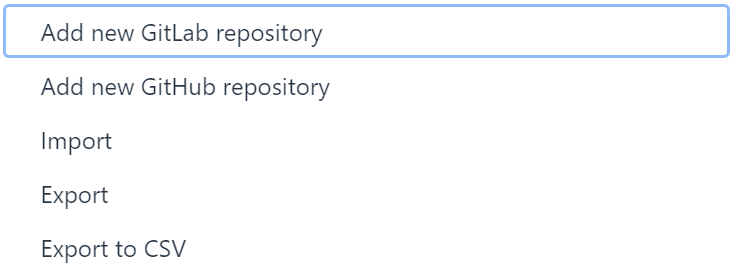
\includegraphics[width=\linewidth]{AnexE-MN-Fig5-1}
		\caption{Menú: ``\textit{Project management}''}
		\label{fig:AnexE-MN-Fig5-1}
	\end{subfigure}\hfill
	\begin{subfigure}{.45\textwidth}
		\centering
		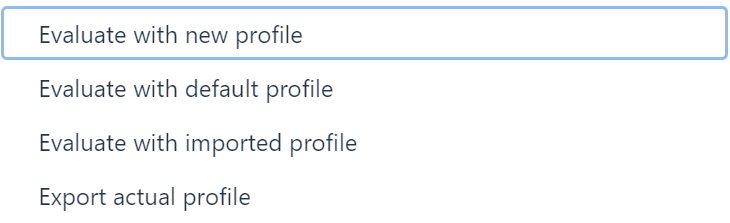
\includegraphics[width=\linewidth]{AnexE-MN-Fig5-2}
		\caption{Menú: ``\textit{Evaluate projects}''}
		\label{fig:AnexE-MN-Fig5-2}
	\end{subfigure}
	\caption{Menús del listado de repositorios}
	\label{fig:AnexE-MN-Fig5}
\end{figure}

La \textbf{tabla} muestra los valores medidos de las métricas para cada proyecto, ver figura \ref{fig:AnexE-MN-Fig8}.

\imagen{AnexE-MN-Fig8}{Tabla que muestra los valores medidos de las métricas para cada proyecto}

Nótese que se tienen los resultados sin conexiones ya que se han importado por archivo.\\
La tabla presenta las siguientes columnas:
\begin{itemize}
	\item \textbf{Botón de eliminar.} Permite eliminar de la tabla el proyecto seleccionado.
	
	\item \textbf{\textit{Project}.} Nombre del proyecto con enlace a su repositorio en su forja. Si el nombre es demasiado largo, éste se corta y para verlo completo se puede utilizar el \textit{tooltip} que aparece al pasar el ratón por encima del nombre del proyecto. Puede que el enlace no funcione si el proyecto se ha eliminado o si no se tienen los permisos de acceso según la conexión correspondiente (\textit{GitHub} o \textit{GitLab}.
	
	\item \textbf{\textit{Date}.} Fecha de la última vez que se obtuvieron las métricas del proyecto.
	
	\item \textbf{Métricas.} Valor medido de las métricas y un color que evalúa la medida en relación a un perfil de métricas.\\
	Las métricas están clasificadas por categoría: Proceso de orientación (\textit{Process Orientation}), Constantes de tiempo (\textit{Time Constraints}) e integración y despliegue continuos (\textit{CICD})\\
	En la cabecera se muestra el nombre de la métrica pero aparecerá la descripción en forma de \textit{tooltip} al pasar el puntero del ratón por encima del nombre.
	Un \textbf{\underline{perfil de métricas}} es un conjunto de valores mínimo y máximo definidos para cada métrica. Los valores que se encuentran debajo de cada nombre de las métricas en la cabecera son sus valores mínimo y máximo separados por un guión. En el \textit{tooltip} se muestra el valor mínimo como Q1 y el valor máximo cómo Q3.
	
	\item \textbf{Botón de recalcular métricas.} Permite volver a obtener las métricas del proyecto (si es posible según la conexión actual a \textit{GitLab} de la aplicación) y evaluar las nuevas métricas de acuerdo al perfil actual. Se mostrará un mensaje de aviso si se han recalculado correctamente y un mensaje de error en caso contrario.
\end{itemize}


\subsubsection{Añadir un proyecto}
Para añadir un nuevo proyecto, el tipo de conexión deberá ser distinto de ``Sin conexión'' (\textit{No connection to GitLab}), es decir que debe haber una conexión. Seleccionar la opción ``\textit{Add new}'' del menú ``\textit{Project management}'', ver figura \ref{fig:AnexE-MN-Fig5-1}. Se abrirá un diálogo como el de la figura \ref{fig:AnexE-MN-Fig6}. Para \underline{cancelar} se puede pulsar \textit{Esc} o hacer clic fuera del diálogo.
\begin{figure}[!h]
	\centering
	\begin{subfigure}{.45\textwidth}
		\centering
		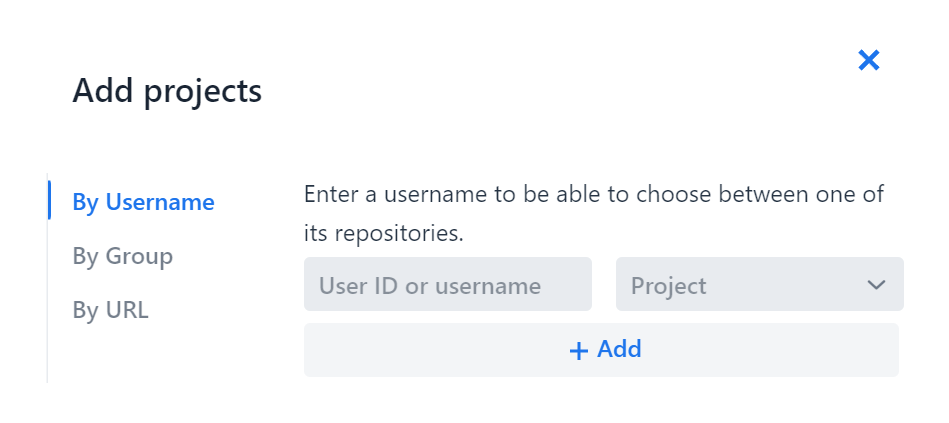
\includegraphics[width=\linewidth]{AnexE-MN-Fig6-1}
		\caption{Menú: ``\textit{Añadir por pertenencia a usuario}''}
		\label{fig:AnexE-MN-Fig6-1}
	\end{subfigure}\hfill
	\begin{subfigure}{.45\textwidth}
		\centering
		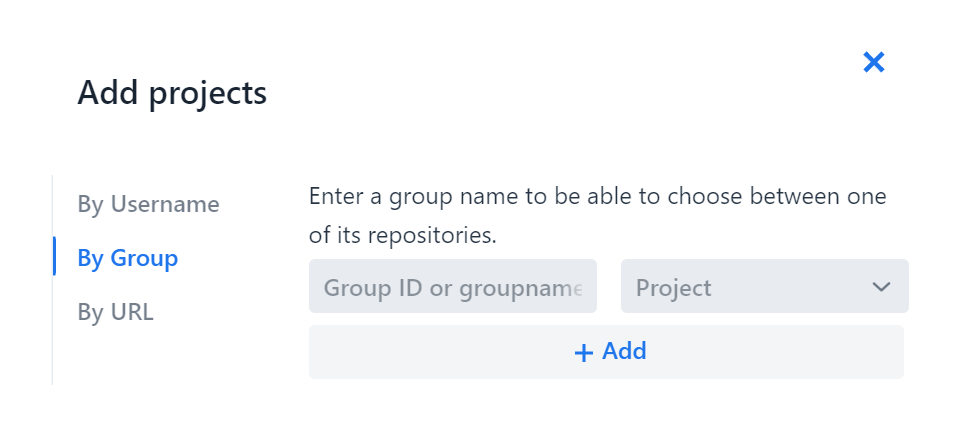
\includegraphics[width=\linewidth]{AnexE-MN-Fig6-2}
		\caption{Menú: ``\textit{Añadir por pertenencia a grupo}''}
		\label{fig:AnexE-MN-Fig6-2}
	\end{subfigure}
	\begin{subfigure}{.45\textwidth}
		\centering
		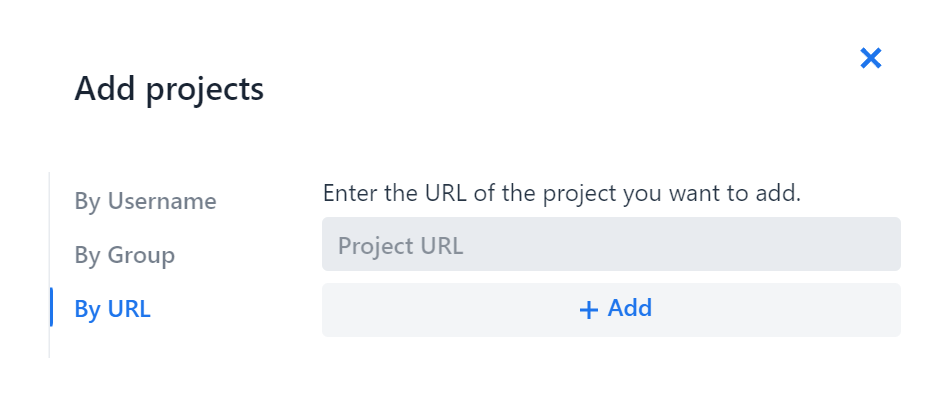
\includegraphics[width=\linewidth]{AnexE-MN-Fig6-3}
		\caption{Menú: ``\textit{Añadir proyecto mediante su URL Web}''}
		\label{fig:AnexE-MN-Fig6-3}
	\end{subfigure}
	\caption{Menús del listado de repositorios}
	\label{fig:AnexE-MN-Fig6}
\end{figure}
Existen tres posibilidades para añadir un proyecto:
\begin{description}
	\item[Añadir por pertenencia a un usuario.] Se solicita en el campo izquierdo del formulario el nombre de usuario o su ID de \textit{GitLab} del cual se desean cargar los proyectos en campo desplegable de la derecha. Se mostrará un mensaje en rojo si el usuario no se existe ``\textit{User not found}'' y un mensaje si el usuario existe ``\textit{User found}'', en ese caso se cargarán todos los proyectos del usuario en el desplegable de la derecha. Seleccionar uno de sus proyectos y pulsar sobre el botón ``\textit{Add}''. Se mostrarán los repositorios públicos (incluyendo \textit{forks}) del usuario. No se mostrarán proyectos privados a menos que se haya establecido una conexión con sesión y el usuario especificado en el campo de la izquierda coincida con el usuario que haya iniciado sesión.
	\item[Añadir por pertenencia a un grupo.] El funcionamiento es el mismo que en el caso anterior, con la diferencia de que se solicita el nombre de grupo o ID del grupo en el campo izquierdo. Si el grupo es privado y el tipo de conexión es pública o el usuario que haya iniciado sesión no tiene acceso al grupo, se mostrará un mensaje en rojo de la misma forma que si el grupo no existiera ``\textit{Group not found}''. Si se encuentra el grupo, se mostrará el mensaje ``\textit{Group found}'' y se cargarán todos los proyectos del usuario en el desplegable de la derecha. Seleccionar uno de sus proyectos y pulsar sobre el botón ``\textit{Add}''.
	\item[Añadir por URL Web.] Se solicita la URL Web del proyecto de \textit{GitLab}. Si no se encuentra, ya sea porque no existe o por la conexión actual, se mostrará un mensaje en rojo al pulsar sobre ``\textbf{\textit{Add}}'': ``\textit{Project not found. It doesn't exists or may be inaccessible due to your connection level.}''
\end{description}

Al añadir un nuevo proyecto, se calcularán por primera vez sus métricas y se evaluarán de acuerdo al perfil de métricas actual. Si no se ha creado o importado ningún perfil, se evaluará según el perfil por defecto.

No se permite volver a añadir un proyecto existente a la tabla.

\subsubsection{Eliminar un proyecto}

Para eliminar un proyecto basta con identificarlo en la tabla y pulsar sobre el icono de basura correspondiente, situado a la izquierda de la tabla. \textbf{Atención}: \underline{NO} se pide confirmación de eliminación.

\subsubsection{Recalcular métricas de un proyecto}

Para recalcular las métricas de un proyecto debe haber una conexión a la forja correspondiente y esta debe tener permisos sobre el proyecto deseado (si es un proyecto privado, debe haber iniciado sesión una persona con permisos de lectura sobre el proyecto). Cumpliendo esos requisitos, solo hay que identificar el proyecto y pulsar sobre el botón correspondiente de recalcular, situado en la parte derecha de la tabla.

\subsubsection{Importar proyectos}
Los proyectos se pueden importar independientemente del tipo de conexión que exista. Se mostrará un diálogo que permite seleccionar o arrastrar al cuadro un fichero con formato \textit{.emr}, ver figura \ref{fig:AnexE-MN-Fig7}. Se puede seleccionar otro fichero en caso de haber escogido un fichero no deseado. Una vez se cargue el fichero, pulsar sobre ``Import''. Se mostrará un mensaje de error en caso de que el fichero este corrompido (ha sido modificado por una herramienta externa a la aplicación), lo que indica que el fichero no podrá volver a utilizarse.
\begin{figure}[!h]
	\centering
	\begin{subfigure}{.45\textwidth}
		\centering
		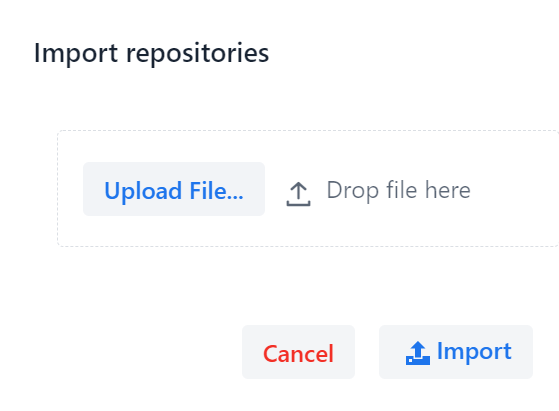
\includegraphics[width=\linewidth]{AnexE-MN-Fig7-1}
		\caption{Diálogo para importar repositorios}
		\label{fig:AnexE-MN-Fig7-1}
	\end{subfigure}\hfill
	\begin{subfigure}{.45\textwidth}
		\centering
		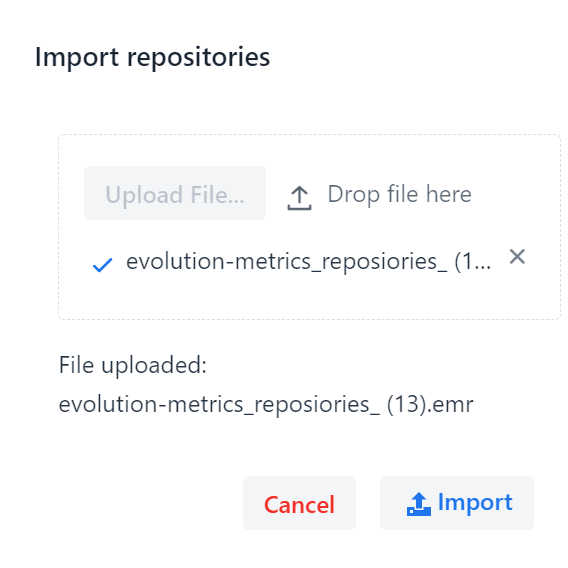
\includegraphics[width=\linewidth]{AnexE-MN-Fig7-2}
		\caption{Diálogo de importar con fichero cargado}
		\label{fig:AnexE-MN-Fig7-2}
	\end{subfigure}
	\caption{Diálogo para importar repositorios}
	\label{fig:AnexE-MN-Fig7}
\end{figure}

Al pulsar sobre ``Import'' puede ocurrir:
\begin{itemize}
	\item Que no haya ningún proyecto en la tabla, entonces se importarán todos los proyecto del fichero.
	\item Que haya algún proyecto en la tabla, entonces se preguntará si se desea añadir los proyecto al listado actual (``Append''); o sobrescribir el listado actual con los proyecto del fichero (``Overwrite''), en ese casó se borrará el listado actual y se añadirán los proyecto del fichero).\\
	En ningún caso se permite añadir proyectos que ya están en la tabla. En caso de que el fichero contenga proyectos existentes, prevalecerán los de la tabla en caso de seleccionar ``Append''.
\end{itemize}


\subsubsection{Exportar proyectos}
Para exportar proyectos debe haber al menos un proyecto en la tabla.
Se puede exportar a un fichero \textit{.emr} para su posterior importación o en un fichero \textit{.csv}. Para exportar hay que seleccionar la opción correspondiente en el menú ``\textit{Project management}'', ver figura \ref{fig:AnexE-MN-Fig5-1}. El dialogo para la exportación se muestra en la figura \ref{fig:AnexE-MN-Fig9}. Basta con pulsar sobre ``\textit{Download}'' para poder descargar el fichero.
\begin{figure}[!h]
	\centering
	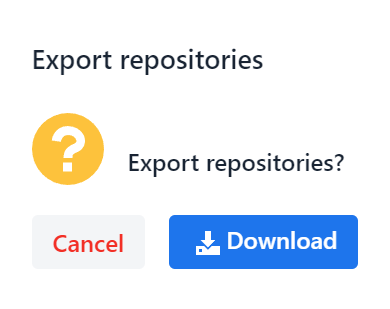
\includegraphics[scale=0.7]{AnexE-MN-Fig9}
	\caption{Diálogo de exportación}\label{fig:AnexE-MN-Fig9}
\end{figure}
\FloatBarrier

También podemos descargarlos en formato \textit{CSV} como se ha indicado anteriormente como se puede ver en la figura: \ref{fig:AnexE-MN-Fig10}.
\begin{figure}[!h]
	\centering
	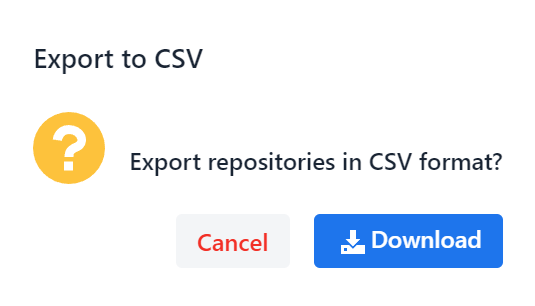
\includegraphics[scale=0.7]{AnexE-MN-Fig10}
	\caption{Diálogo de exportación como \textit{CSV}}\label{fig:AnexE-MN-Fig10}
\end{figure}
\FloatBarrier


\subsubsection{Evaluar los proyectos}
Evaluar un proyecto es comparar las métricas que se han medido de los proyectos en relación a un perfil de métricas en el que se definen los valores mínimos y máximos de cada métrica. El resultado de la evaluación puede ser bueno (la medida se pinta en verde en la tabla), malo (la medida se pinta en rojo) o ``advertencia'' (la medida equivale al valor mínimo o al valor máximo).

Para evaluar los proyectos (se evalúan todos) hay que elegir el perfil de métricas con el que se va a evaluar. Por defecto se coge un perfil de métricas en el que los valores mínimos se corresponden con los cuartiles Q1 y los valores máximos con cuartiles Q3 de un conjunto de medidas tomadas sobre otros TFGs \footnote{\url{https://github.com/clopezno/clopezno.github.io/blob/master/agile_practices_experiment/DataSet_EvolutionSoftwareMetrics_FYP.csv}}. Se puede elegir otro perfil de métricas según la opción elegida en el menú ``\textit{Evaluate projects}'' de la figura \ref{fig:AnexE-MN-Fig5-2}:
\begin{itemize}
	\item \textbf{\textit{Evaluate with new profile}.} Coge como entrada todas las medidas de la tabla y calcula, por cada métrica, los cuartiles Q1 y Q3 y los define como valor mínimo y valor máximo de la métrica.
	\item \textbf{\textit{Evaluate with default profile}.} Permite evaluar los proyectos con el perfil por defecto mencionado anteriormente.
	\item \textbf{\textit{Evaluate with imported profile}.} Permite importar el perfil de métricas de un fichero \textit{.emmp}. El perfil se debe haber creado y exportado anteriormente.
\end{itemize}

Las métricas se evalúan como buenas si:
\begin{itemize}
	\item I1: El valor medido supera el umbral mínimo (Q1).
	\item I2: El valor medido se encuentra entre el umbral mínimo y el máximo (Q3).
	\item I3: El valor medido supera el umbral mínimo.
	\item TI1: El valor medido se encuentra entre el umbral mínimo y el máximo.
	\item TC1: El valor medido se encuentra entre el umbral mínimo y el máximo.
	\item TC2: El valor medido se encuentra entre el umbral mínimo y el máximo.
	\item TC3: El valor medido se encuentra entre el umbral mínimo y el máximo.
	\item C1: El valor medido se encuentra entre el umbral mínimo y el máximo.
	\item IC1: El valor medido se encuentra entre el umbral mínimo y el máximo. Si es el valor es 0 el proyecto no tiene integración y despliegue continuo.
	\item IC2: El valor medido se encuentra entre el umbral mínimo y el máximo Si es el valor es 0 el proyecto no tiene integración y despliegue continuo.
	\item IC3: El valor medido se encuentra entre el umbral mínimo y el máximo Si es el valor es 0 el proyecto no tiene integración y despliegue continuo.
	\item DC1: El valor medido se encuentra entre el umbral mínimo y el máximo Si es el valor es 0 el proyecto aún no tiene ninguna \textit{release}.
	\item DC2: El valor medido se encuentra entre el umbral mínimo y el máximo.
\end{itemize}

Junto con las métricas se proporciona un indicador (\textit{Calif.}) del porcentaje de las mismas que se han evaluado como buenas (en verde).

\subsubsection{Exportar perfil de métricas}
Se puede exportar el perfil de métricas a un fichero \textit{.emmp} para su posterior importación. Para ello, seleccionar la opción correspondiente del menú ``\textit{Evaluate projects}'' de la figura \ref{fig:AnexE-MN-Fig5-2}: ``\textit{Export actual profile}''. El diálogo para la exportación es similar al de la figura \ref{fig:AnexE-MN-Fig9}. Basta con pulsar sobre ``\textit{Download}'' para poder descargar el fichero que contendrá el perfil de métricas actual.